\documentclass{article}
\usepackage[UTF8]{ctex}
\usepackage{geometry}
\usepackage[colorlinks,linkcolor=red]{hyperref}
\usepackage{natbib}
\geometry{left=3.18cm,right=3.18cm,top=2.54cm,bottom=2.54cm}
\usepackage{graphicx}
\pagestyle{plain}	
\usepackage{setspace}
\usepackage{caption2}
\usepackage{datetime} %日期
\usepackage[colorlinks,
            linkcolor=black,
            anchorcolor=black,
            citecolor=black
            ]{hyperref}
\renewcommand{\today}{\number\year 年 \number\month 月 \number\day 日}
\renewcommand{\captionlabelfont}{\small}
\renewcommand{\captionfont}{\small}
\begin{document}

\begin{figure}
    \centering
    
\includegraphics[width=8cm]{upc.png}

    \label{figupc}
\end{figure}

	\begin{center}
		\quad \\
		\quad \\
		\heiti \fontsize{45}{17} \quad \quad \quad 
		\vskip 1.5cm
		\heiti \zihao{2} 《计算科学导论》课程总结报告
	\end{center}
	\vskip 2.0cm
		
	\begin{quotation}
% 	\begin{center}
		\doublespacing
		
        \zihao{4}\par\setlength\parindent{7em}
		\quad 

		学生姓名:\underline{\qquad  侯鹏辉 \qquad \qquad}

		学\hspace{0.61cm} 号:\underline{\qquad 1907010117\qquad}
		
		专业班级:\underline{\qquad 计科1901 \qquad  }
		
        学\hspace{0.61cm} 院:\underline{计算机科学与技术学院}
% 	\end{center}
		\vskip 2cm
		\centering
		\begin{table}[h]
            \centering 
            \zihao{4}
            \begin{tabular}{|c|c|c|c|c|c|c|}
            % 这里的rl 与表格对应可以看到,姓名是r,右对齐的;学号是l,左对齐的;若想居中,使用c关键字。
                \hline
                课程认识 & 问题思 考 & 格式规范  & IT工具  & Latex附加  & 总分 & 评阅教师 \\
                30\% & 30\% & 20\% & 20\% & 10\% &  &  \\
                \hline
                 & & & & & &\\
                & & & & & &\\
                \hline
            \end{tabular}
        \end{table}
		\vskip 2cm
		\today
	\end{quotation}

\thispagestyle{empty}
\newpage
\setcounter{page}{1}
% 在这之前是封面,在这之后是正文
\section{引言}
转眼间,一个学期已经快要过去。相比较刚刚入学时,对计算机一窍不通的我来说,现在的我已经对计算机这片领域有所了解了,尤其是在经过计算机科学导论学习之后,使得我对计算机的历史及其组成有了深刻的理解。尽管,计算机科学导论这门课对于一个理科生来说,跟偏向于文科或者说更偏向于哲学。因此,这边要看老师的功底了,看老师是否能将这门学科讲活。说实话在上这门课之前,就有很多同学说这是一门水课,我其实并不怎么想放过的,但是当我们宿舍的大佬的也这样说甚至这样做的时候,我确实便想也水一下就过去了。但是,后来老师布置的任务,却让我不得不听一下这课的内容,尽管对于理科的我很是有些困意,但是我发现,老师讲的内容有些确实很是惊奇,也是我所需要的内容。我想这时已经不能跟随大众了,因为这门课确实很有作用,并且在学完一学期之后,我也确实很有收获。像对于计算机的发展史有了较为基础的认识。并且不限于此,老师的讲课方式让我也了解了众多课外的知识,类似于JavaScript等等,尽然之前有几节没有认真听。但是好在我之后还是有在好好听课,这让我获益匪浅。\par

\section{对计算科学导论这门课程的认识、体会}
如上述,计算机科学导论这门课对于一个理科生来说,跟偏向于文科或者说更偏向于哲学,但是这对于一个想成为“大牛”得技术人员来说是必不可少的,当从思想上得到触发时,你所创造的东西会变得多起来,对了一件事物,一段代码的认识也会深刻起来,更重要的是,对于他的迁移转化会更加新奇别致巧妙。虽然我还领悟到精髓,但是我想继续对于计算机科学导论的学习会令我的想法更加多且合理,这是这门课的独特恩泽。让我不仅仅是一个代码的搬运工或代码的输出极,而是一个有着自己想法的人。会给之后的更加深入的学习打下基础。\par

\section{Harmony OS}

\subsection{缘由}
因为之前只知道学习的事,并且很少接触外界,所以对一切都不怎么清楚,受高考考时事政治的影响,所以会每周都看《新闻周刊》,就在去年频繁出现在新闻周刊中的一个词,就是中美贸易战。而在这场战贸易战中,华为又是出现最多的。我在想,这是一个国家要针对这个企业么?还是一个目前居于世界极其前列的位置的超级大国,受到如此针对应该会想前段时间的中兴一样,事后只能苟延残喘了吧。毕竟这是一个不可抗拒的力量了。然而,先是海思在芯片供应不足时力挺华为,后来,连Google的Android也有可能不能使用过,这还不完?尽管不太了解操作系统是什么,但是知道他是一个十分重要的东西,对于手机来说。而当我听说有个叫鸿蒙操作系统的东西可以帮助华为渡过难关。我心想华为这运气也忒好了吧,要是没有这么多公司的帮助,恐怕已经凉了。\par
然而,后来我听说,海思是华为的子公司,鸿蒙操作系统是华为的研发室研发的。我彻底震惊了,这该是多么的未雨绸缪之态才能做到这种地步。能让一个超级大国都束手无策,甚至了解到就连美国的Google公司也是极力请求政府能够免除禁令,甚至有报道黑名单已经伤害了美国公司例如数据存储制造商美光科技公司和半导体生产商博通公司。 \cite{ref1}
这连敌人的队友都变阵了,既让我啼笑皆非,又让我深深的认识到华为的厉害之处,由此,我想了解一下华为,便从harmonyOS入手。\par
\newpage
\subsection{由来}
\begin{enumerate}
    \item [ ]混沌未分天地乱,茫茫渺渺无人见。
    \item [ ]自从盘古破鸿蒙,开辟从兹清浊辨。
    \item [ ]覆载群生仰至仁,发明万物皆成善。
    \item [ ]欲知造化会元功,须看西游释厄传。
\end{enumerate} \par
这段西游记第一回的“灵根育孕源流出 心性修持大道生”是鸿蒙的相关处之一。可见鸿蒙这个名词就有着悠长的历史。\par
鸿蒙操作系统的历史由来也有些年头。这得从2002年说起,当时的华为真是的到了破产的地步“2002年开干部大会是在IT泡沫破灭,华为濒于破产、信心低下的时候召开的”,“那时世界处在困难时期,而华为处在困难的困难时期”最终他殊死一搏,显然博成功了。 \cite{ref2}
而那次的博,也确立了华为的总战略,确立出了华为将会像一只大乌龟一样,一心一意专心致志的爬着自己的旅途,心无旁骛。不久海思成立了。\par 
2009 华为成立编译组,秘密研发,只在自研芯片,新一代通信 ,云计算,操作系统,等技术提供编译器的基础设施。\par
2012 代号”2012实验室“深入技术研究。并衍生出多个实验室,类似诺亚方舟实验室、欧拉实验室、香农实验室、高斯实验室。其中令国人精神大振的鸿蒙操作系统就是出自于欧拉实验室,而方舟编译器,其实出自于诺亚方舟实验室。\par
2012 任正非提出:“(如果)Android 系统不给我用了,Windows Phone 8 系统也不给我用了,我们是不是就傻了?期初还有人嘲笑他,即便说得很有道理,但是,在当时的情况下,这样的情况也轮不到你家华为来考虑。\par
2019年8月9日的HDC大会上余承东正式宣布发布鸿蒙操作系统。\par 
\subsection{操作系统}
要研究鸿蒙操作系统,首先要了解什么是操作系统。\par
操作系统是什么呢?硬件之上软件之下的位置,即可管理硬件(像 内存、硬盘、CPU之类的)又可管理应用程序(系统进程之类),举个例子吧,像Linux(这一族开发者众多,发行版本以千计,覆盖所有平台,并支持所有文件格式和所有网络协议)、FreeBSD、Windows,Mac,Android(我们平常非苹果手机使用的便是这个)等等,可谓种类众多。一般可以根据使用端来分类。手机端有 android (安卓),ios(苹果) ,windows phone,windows mobile,Symbian(诺基亚),BlackBerry OS(黑莓)而PC(即电脑)有linus,windows,mac(苹果PC端),dos ,freebsd,unix,chromeos等等。\par
同时操作系统的组成有两大构件:内核与外核。通常的操作系统内核与外核都是集中在一起的,这样可以大大优化,进程之间的切换速度。所以,像基于Linux的安卓等这类的大厂都是采用的宏内核为主要框架,为作为微内核windows却只能用于电脑端,而半道出家的混合式内核架构IOS(苹果的的手机端)也并非完全是微内核。这时鸿蒙OS便出现了,全球第一个基于微内核的全场景分布式操作系统。\par 
\subsection{构成}
\begin{enumerate}
    \item []底层内核(Linux内核、鸿蒙微内核、LiteOS)的混合内核。
    \item []基础服务(多Run Time如方舟等、通用系统服务、IoT设备专有服务、分布式数据管理、虚拟外设、UI图形、分布式软总线)。
    \item []程序框架(多用户程序框架如鸿蒙、Web……)。
    \item []应用(手表应用、大屏应用、车机应用、PC应用)。
    \item []另外,础服务将设为外核,新增文件系统、电源管理、内存管理与设备驱动,内核为鸿蒙微内核。
\end{enumerate}
\subsection{优势}
虽然目前鸿蒙操作系统是混合内核 (linus + liteOS + 鸿蒙内核),但如果鸿蒙OS作为一款微内核的手机操作系统的话,能引起这么大的关注必然有它的独特之处。\par
\begin{enumerate}
    \item {分布式架构首次用于终端OS,实现跨终端无缝协同体验,即可以在所有设备上无缝连接。鸿蒙OS采用“分布式OS架构”和“分布式软总线技术”,通过公共通信平台、分布式数据管理、分布式能力调度和虚拟外设四大能力,将相应分布式应用的底层技术实现难度对应用开发者屏蔽,使开发者能够聚焦自身业务逻辑,像开发同一终端一样开发跨终端分布式应用,也使最终消费者享受到强大的跨终端业务协同能力为各使用场景带来的无缝体验。}
    \item {流畅和高性能(相较于安卓能快40\%甚至到60\%),这得归功于确定时延引擎和高性能IPC技术而实现了系统天生流畅。首先,确定时延引擎可在任务执行前分配系统中任务执行优先级及时限进行调度处理,优先级高的任务资源将优先保障调度,应用响应时延降低25.7\%。其次,鸿蒙微内核结构小巧的特性使IPC(进程间通信)性能大大提高,进程通信效率较现有系统提升5倍。另外,其方舟编译器为静态编译器,完美契合确定时延引擎技术。}
    \item {安全性极高,基于微内核架构重塑终端设备可信安全。因为微内核与系统模块的分离,安全模式升级。同时,鸿蒙操作系统使用全新的微内核设计,具有增强的安全性和低延迟。这个微内核旨在简化内核功能,在内核之外的用户模式下实现尽可能多的系统服务,并增加相互安全保护。微内核本身只提供最基本的服务,如线程调度和IPC。并且鸿蒙操作系统的微内核设计使用正式的验证方法,在可信的执行环境(TEE)中,从根本上重塑安全性和可信度。形式化验证方法是从源头验证系统正确性的一种有效的数学方法,而传统的验证方法,如功能验证和攻击仿真,则局限于有限的场景。相比之下,形式化方法可以使用数据模型来验证所有的软件运行路径。另外,鸿蒙操作系统是第一个在设备TEE中使用正式验证的操作系统,大大提高了安全性。此外,由于鸿蒙操作系统微内核的代码要少得多(大约是Linux内核数量的千分之一),所以攻击的概率大大降低了。}
    \item {更重要的是统一的系统,通过统一IDE支撑一次开发,多端部署,实现跨终端生态共享。关于这个,可以归功于华为的方舟编译器,华为方舟编译器是首个取代Android虚拟机模式的静态编译器,可供开发者在开发环境中一次性将高级语言编译为机器码。此外,方舟编译器未来将支持多语言统一编译,可大幅提高开发效率。 \cite{ref3} } 
    \item {还有就是对于鸿蒙操作系统真正的野心,用为物联网时代的多部署。过去开发者为手表开发应用和为手机开发应用不一样,为不同硬件做适配、开发,工作量很大,鸿蒙OS支持开发者一套代码,通过华为提供的开发环境,能够适配不同种类终端,非常方便,一次开发多端部署,提升开发效率,跨设备生态共享。例如音乐播放软件开发,到家里就是大屏,电视上智慧屏,都可以自动适配。鸿蒙OS的IDE环境可以通过拖拽方实现自动适配。}
    \item {这其中的一个强大助力就是方舟编译器。它是一款统一编译器,鸿蒙OS支持的方舟编译器是真正支持多编程语言统一编译器,可以大大提升开发效率,甚至混合编程,高性能程序可能用C++,但是一般应用用JAVA、Kotlin,甚至支持混合编译,大大提升运行程序效率,同时鸿蒙OS借助分布式能力,提供了Kit开发跨终端应用,包括分布式软总线Kit等等,通过Kit实现分布式能力跨终端开发,像开发普通应用一样非常简单。过去操作系统都没有支持这样的能力,现在开发者将得到很大的方便。}
    \item {最最令我钦佩的是华为发布开发者计划鸿蒙OS向全球开发者开源。}
\end{enumerate}
\subsection{发展}
2017年鸿蒙内核1.0完成技术验证.\par
2018年鸿蒙内核2.0用于终端TEE.\par
2019年5月华为被列为“实体清单”(Entity List),Google将只能提供开源的代码, Google Play Store、Google 语音控制助理、Google 地图、Gmail、YouTube 等应用,华为设备虽然可以下载但是将无法正常访问。这确实很让人头疼。\par
2019.5.24 国家知识产权局商标局网站显示,华为已申请“华为鸿蒙”商标,申请日期是 2018 年 8 月 24 日,注册公告日期是 2019 年 5 月 14 日,专用权限期是从 2019 年 5 月 14 日到 2029 年 5 月 13 日。\par 
2019.2.17 有网友曝光由上海陈海波教授领导华为操作系统团队开发的自主产权操作系统「鸿蒙」的相关技术应用。(陈海波教授:上海交大的教授、博导,华为 OS 首席科学家、操作系统内核实验室主任, 曾获奖:“向多核平台的日用操作系统性能可伸缩性研究”(项编号:61003002)“与“教育部-英特尔信息技术专项科研基金项目“多核编程模型的优化及系统软件支持”(项目编号MOE-INTEL-09-04),”) \cite{ref4} \par
2019.8.9 华为开发者大会(HDC) 公开发布鸿蒙。\par
2019.8.10鸿蒙0S 1.0正式使用,荣耀智慧屏(以及pro)正式搭载鸿蒙操作系统。\par 
2020年发计划发布鸿蒙OS 2.0.。其中内核和应用框架实现完全自研,体系上由通用微内核架构、高性能图形栈、支持多语言统一编译、多终端开发IDE并满足车规级标准,落地产品包括创新国产PC、手表/手环、车机\par
2021年之后用于VR和耳机等方面。\par 
\begin{figure}[h]
    \centering
    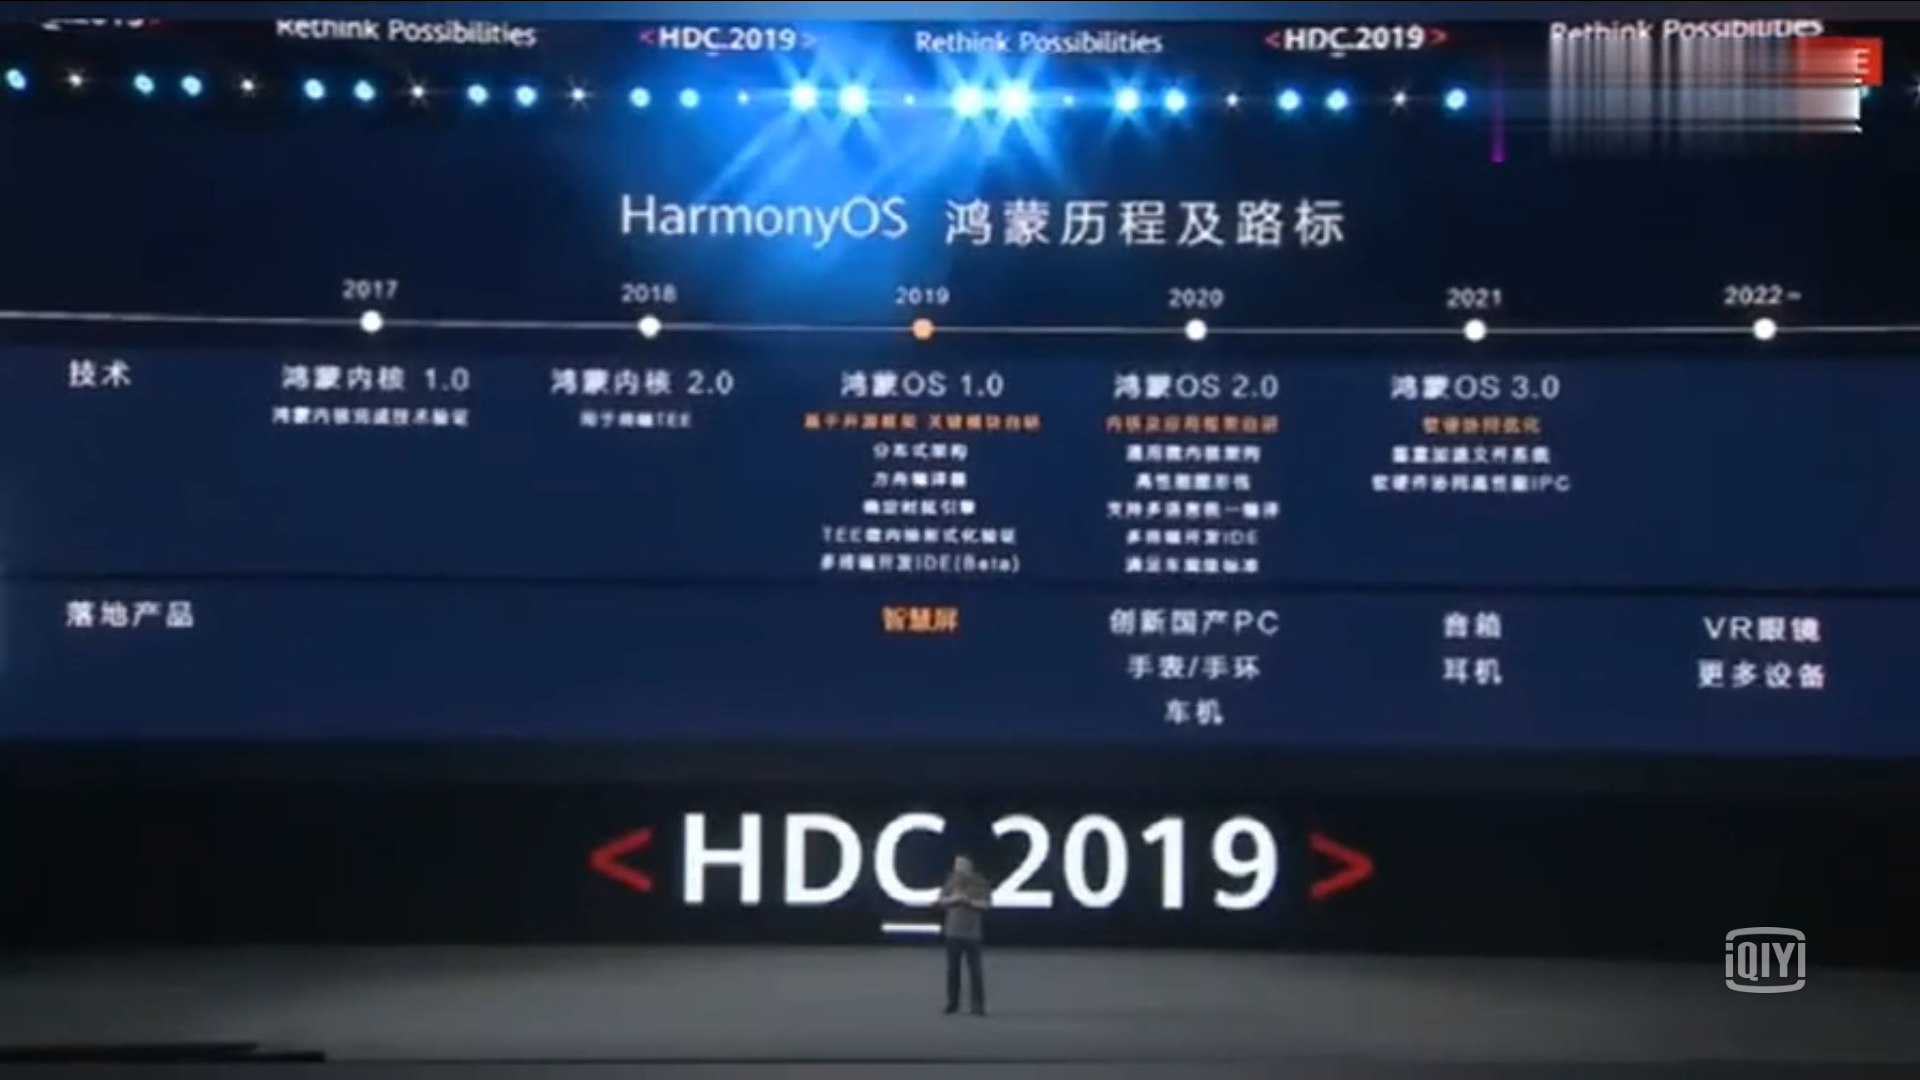
\includegraphics[scale=0.3]{1.1}
    \caption{HDC发布现场}
    \label{fig:1.1}
    \end{figure} \par
    
\subsection{全场景智慧化战略}
鸿蒙操作系统,与其说是手机系统,跟不用说,以手机为起点而搭建的万物物联的系统。这也是他的真正的核心。我想鸿蒙操作系统本来也是为了互联网时代而发明的,知识贸易战碰巧让他提前出现了。因为他的目标不仅局限于手机或PC而是可穿戴设备、智慧屏、车机设备,未来包括工业自动化控制、无人驾驶等,横跨手机、平板、电视、物联网等多个平台的方面,这恰恰是万物互联的方面。\par 
而实际上也确实应该如此,因为这恰巧响应了华为全场景智慧化战略,这个战略概括起来就是1个核心驱动力-华为HiAI;2个生态平台-硬件生态和服务生态;3层结构化产品-1+8+N。其中硬件生态是HUAWEI HiLink平台是华为IoT生态的基础架构,是IoT生态产品互联互通的开放平台。服务生态是Ability Gallery快服务智慧平台帮助开发者实现用更低成本获取更高开发价值,让终端服务向着更加“精准而智慧”发展。而结构化产品-1+8+N,鸿蒙十分契合。(1+8+N解释为“1”是指是以手机为主的入口,以平板、穿戴、HD、PC、耳机、VR、AI音箱、车机这八款在特定场景中常用到的产品为辅助入口,N”是“泛IoT硬件”,包括照明、安防、环境、清扫等,以实现覆盖多个场景。)\par
当然5G与AI(人工智能)也是其中一环,但不多赘述。2019年被业界视为“5G商用元年”,AI+IoT+5G的技术变革与融合,是实现万物互联的催化剂。余承东表示:“我们现在从NB-IoT、Wi-Fi等新的技术到5G连接,真正理解了万物互联。提供芯片、模块、软件支持到开发平台,包括5G,都会让大家用。” \cite{ref5} \par 

\subsection{某些疑惑}
针对于某些人说的一些问题,我简单做出回答。\par
\begin{enumerate}
    \item {有人说华为的生态是一大问题,很难构建。这一点我也是很赞同的,就连任正非也是这样认为的,(“做一个操作系统的技术难度不大,难度大的是生态。”在一次采访中,任正非对第一财经记者表示)。因为之前的一款同样是微内核操作系统的黑莓手机(QNS嵌入式微内核)的前车之鉴还摆在那里,总不能掉以轻心。事实上,我们想到了,任正非也必然想到了。细想一下便可知道,最近华为手机已经更新至EMUI10(Magic3.0)实际上这个操作系统已经有绝大多数的部分是鸿蒙操作系统构成的(据说占比已达75\%),也就是说华为一直以来都在秘密测试鸿蒙操作系统,并且允许鸿蒙与Android系统兼容,就是为了防止鸿蒙系统没有相应的生态,而像WP一样倒下,也就是说如果没有发生贸易战的话,鸿蒙会正常的自然而然的便过度下去,软件本身便会兼容Android,不用过多考虑生态问题。但是贸易战这一个关键点确实令人有些意外,如果真无法兼容,也许华为公司会有一套B方案吧。毕竟队友我们来说,只能是针对国内生态,国内各厂商必然是帮助华为构建生态,但是国外的生态可能需要鸿蒙的人缘,来积攒构建了。}
    \item {也有人问华为应该如何处理过渡问题,之前说了没有贸易战的话会按照之前的计划慢慢过渡。当然现在是不可能了。倘若真的无法兼容Android时势必会失去一些华为粉,但是那时完全解放的鸿蒙的特性相信也会吸引更多用户来使用华为。国内的上文有叙述。\cite{ref6} } 
    \item {另外有一些国外网站评价“2019年8月9日,华为在发布会并未展示鸿蒙操作系统,故鸿蒙系统被网民戏称为“哄懵系统”和“ppt系统””,也确实无可厚非,因为系统还并未开源,但是余承东曾正式宣布harmony OS将会开源,这种事情耐心等待即可,不需要过多的破费口舌。}
 \end{enumerate} \par

\section{总结}
鸿蒙的诞生拉开了永久性改变操作系统全球格局的序幕。\par 
华为的坚强抵抗为中国其他相关制造商提供了喘息的时间,这尤其使华为的屹立不倒具有了全局意义。中国的各家厂商彼此既是竞争者,又组成了一个微妙但却真实的利益共同体。让鸿蒙的生态系统建立起来,这不仅对华为生死攸关,也是中国所有相关制造商未来生存环境的一个决定性砝码。\cite{ref7}\par 
感谢老师能够给予我这个机会,让我有这次机会能够充分了解一下华为与鸿蒙OS,提升了我的知识储量。其实这是我的第二篇,第一份的报告以及规划总共一万三千字多,但是电脑崩了,在最后这天勉强干完第二遍。第一篇写了八千字,而且写的比这次更全面,但是这次写得更有条理,因为时间关系,所以有些精简,但是思路确实是理顺了,而且认识是更加充分了。感谢老师有了这机会。\par
\section{附录}
\begin{itemize}
    \item {
        \bf{Github}\\
        Profile: https://github.com/JKL-gentler\\
        \begin{figure}[h]
            \centering
            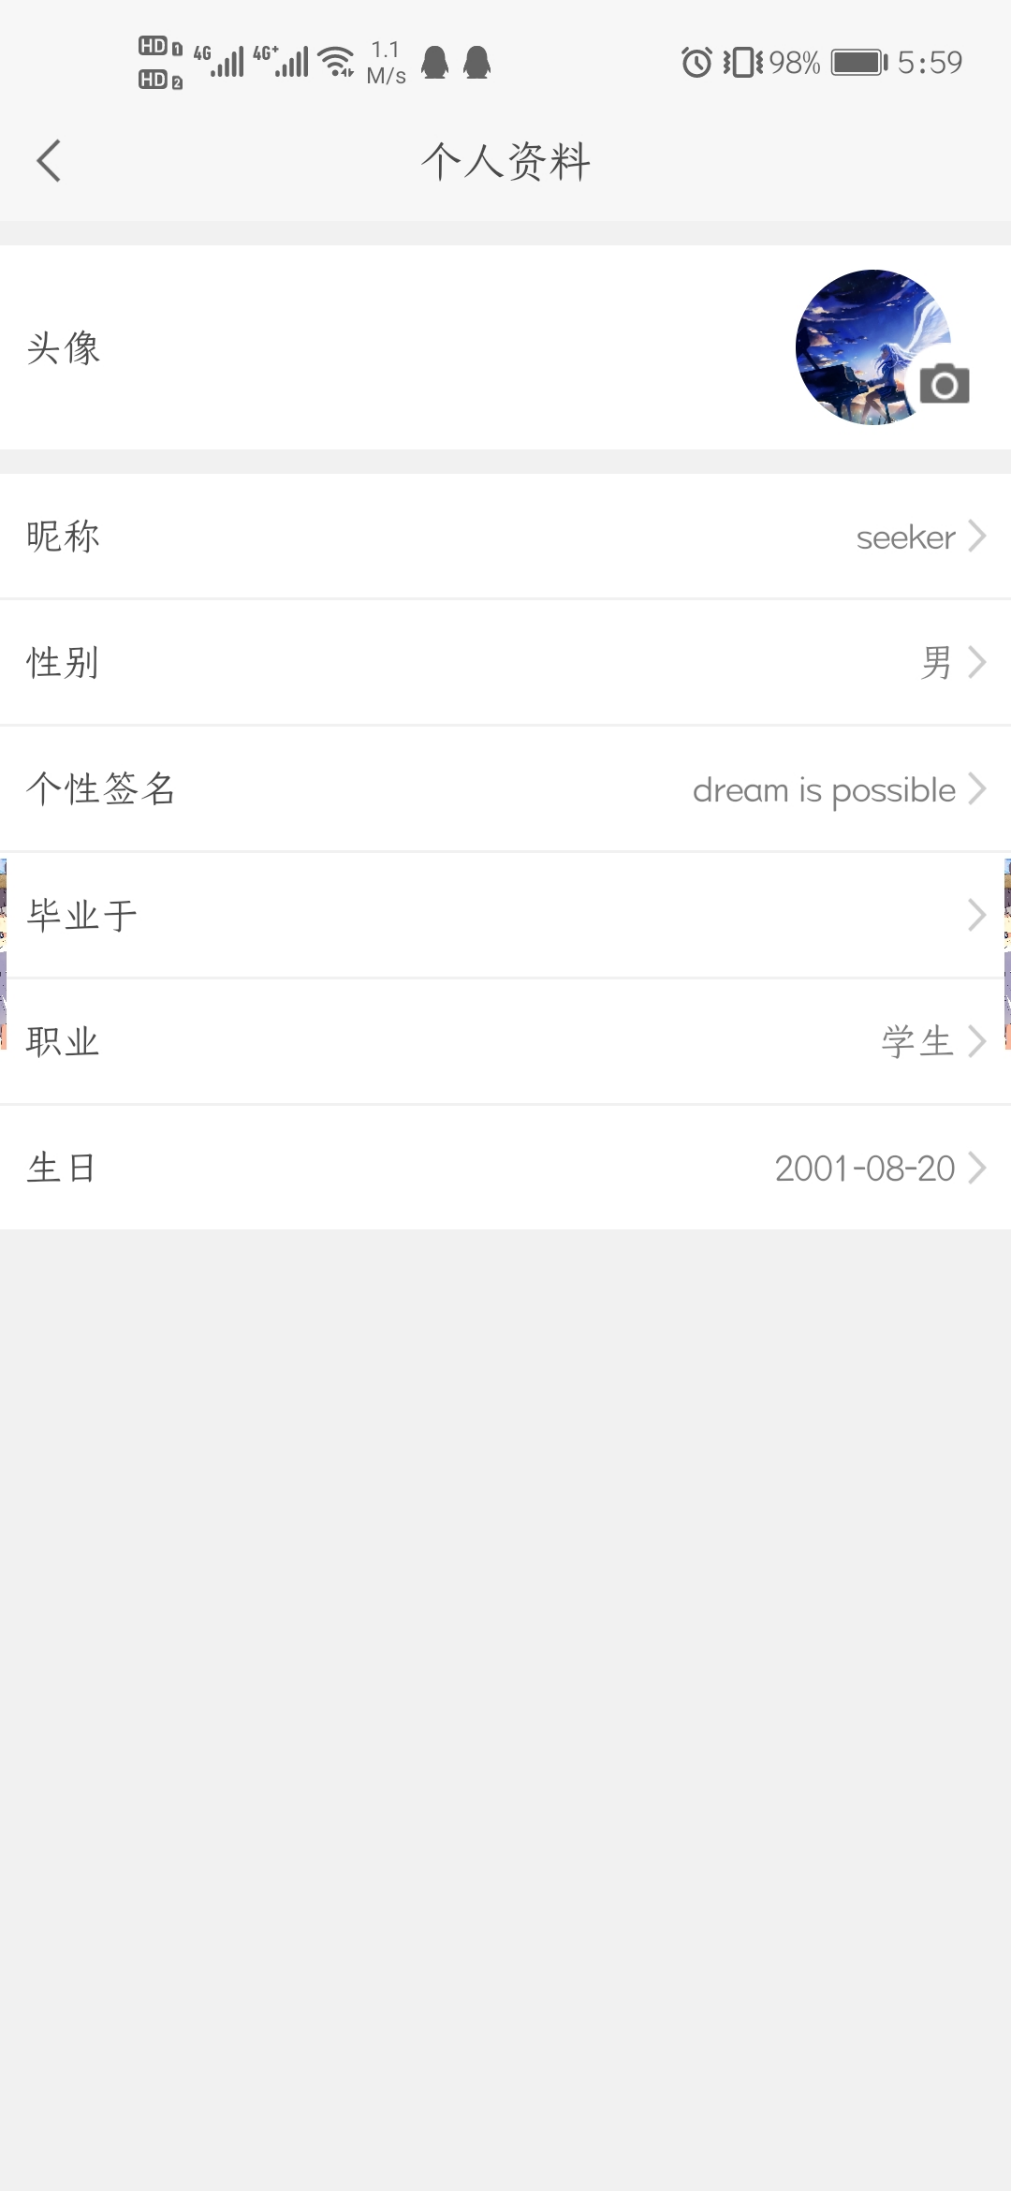
\includegraphics[scale=0.2]{1.3}
            \label{fig:1.2}
        \end{figure}
    }
\newpage
    \item {
        \bf{观察者网}\\
        \begin{figure}[h]
            \centering
            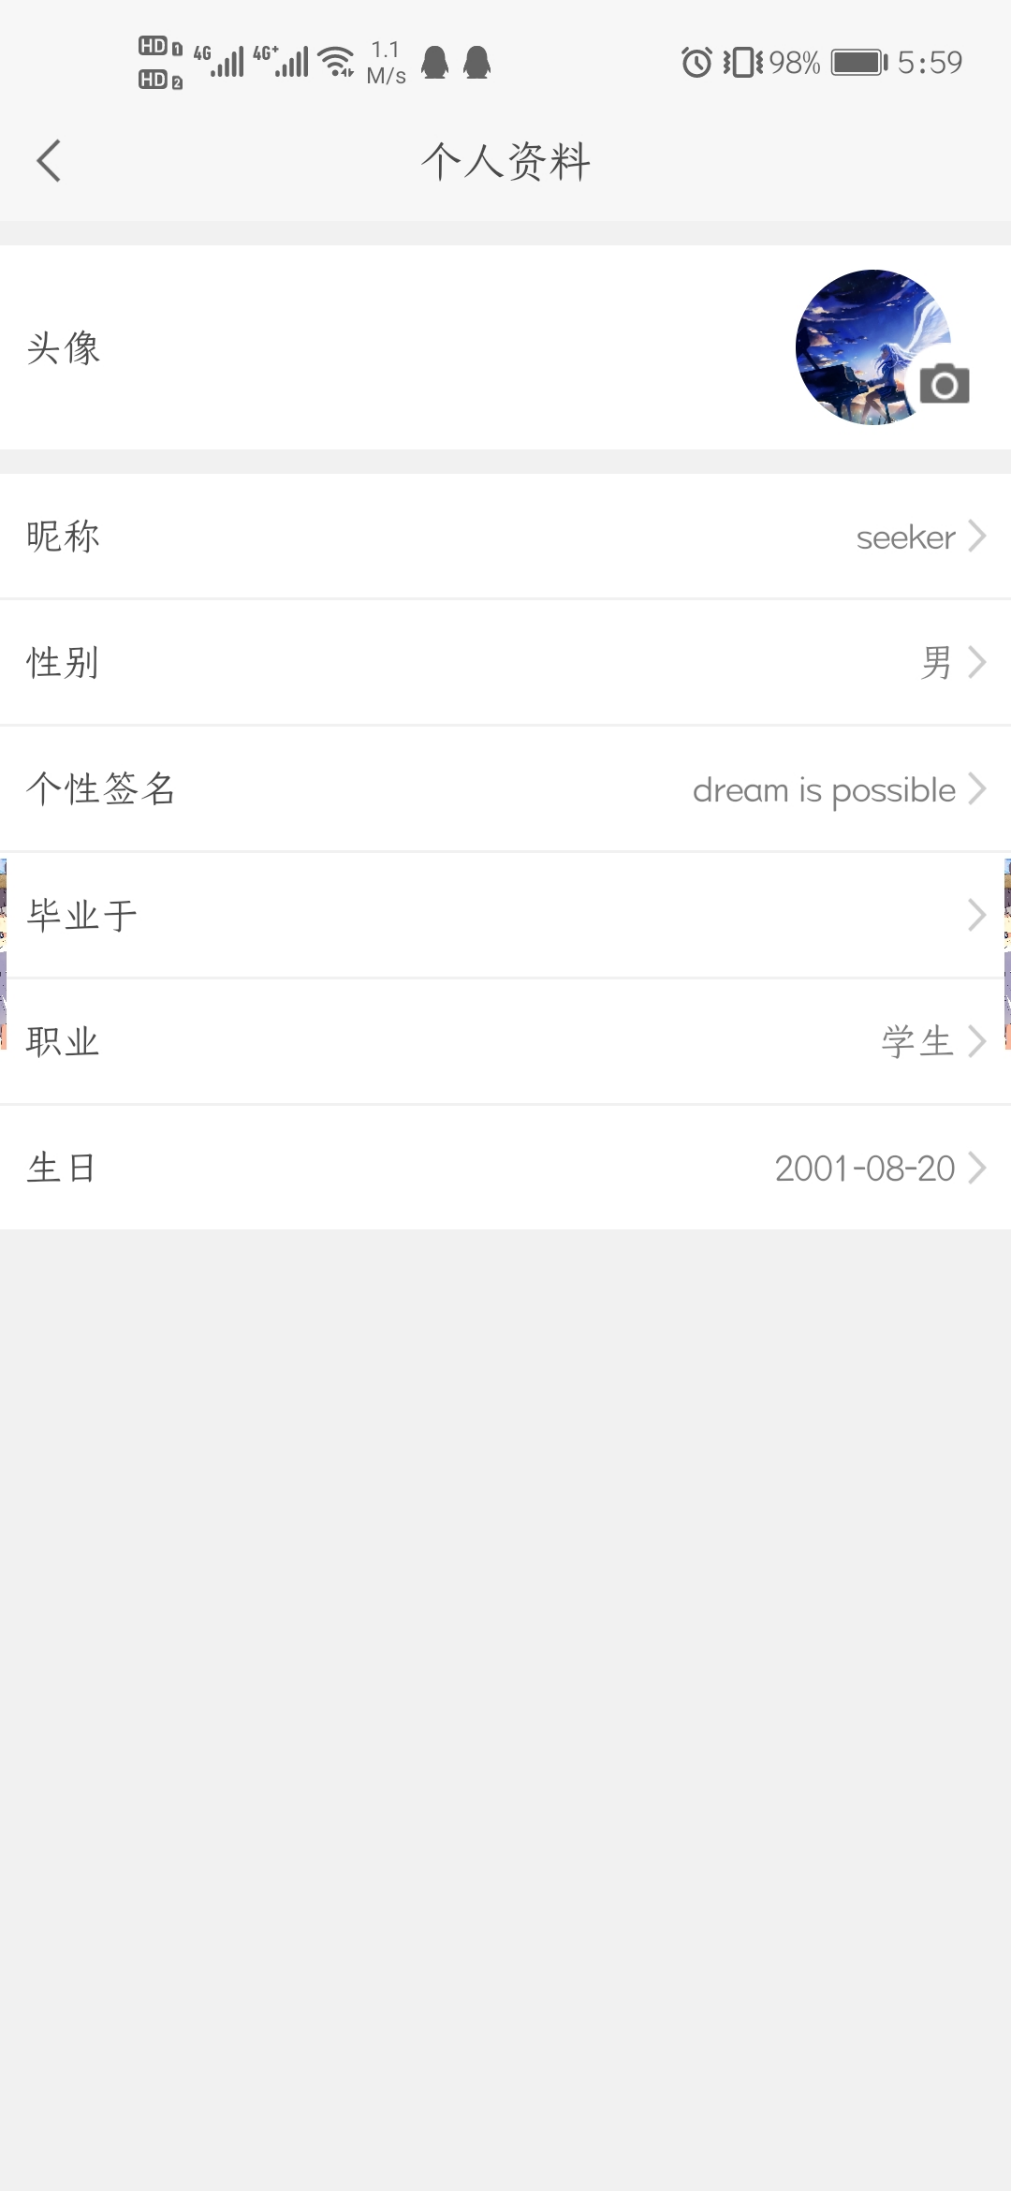
\includegraphics[scale=0.1]{1.3}
            \label{fig:1.3}
        \end{figure}
    }
    \item {
        \bf{学习强国}\\
        \begin{figure}[h]
            \centering
            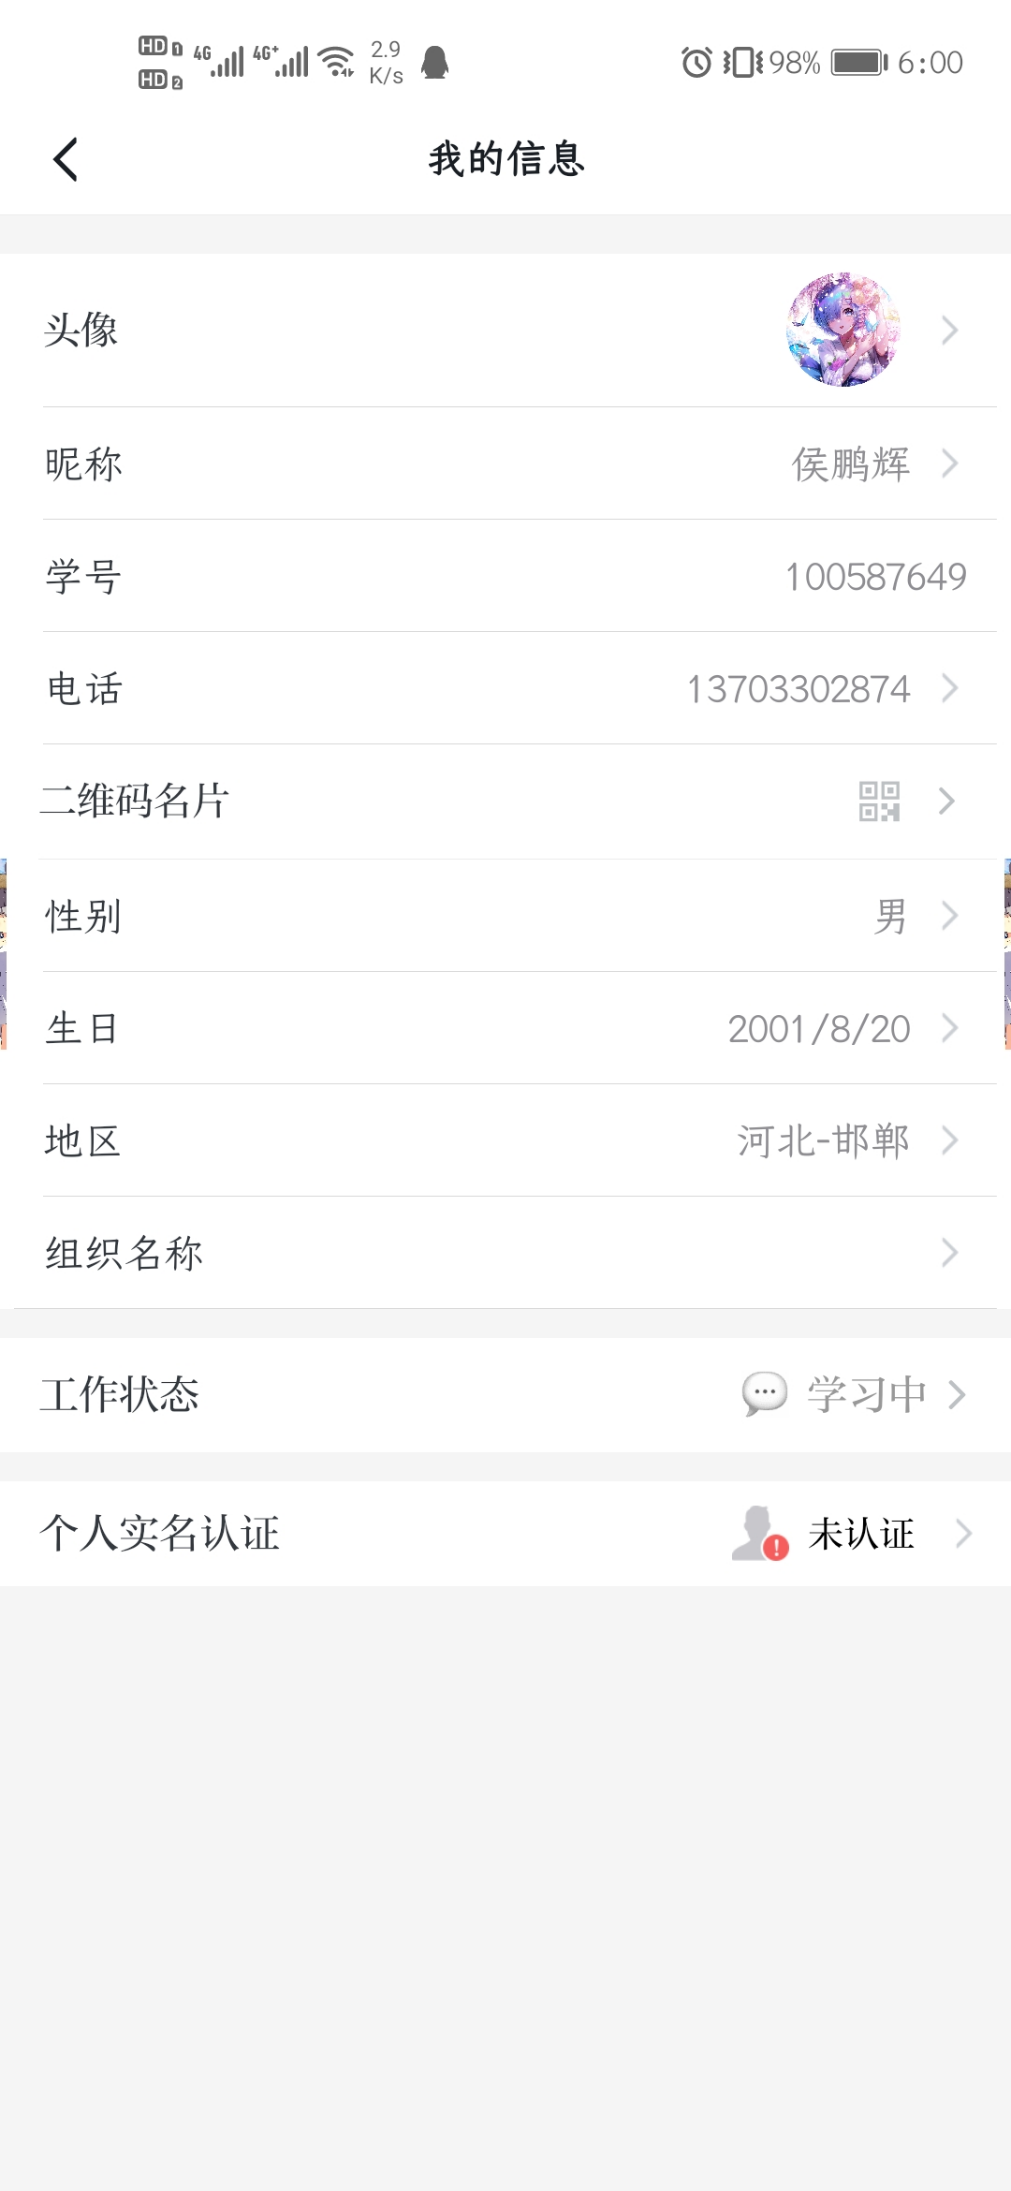
\includegraphics[scale=0.1]{1.4}
            \label{fig:1.4}
        \end{figure}
    }
    \item {
        \bf{bilibili}\\
        Profile: https://space.bilibili.com/396184656\\
        \begin{figure}[h]
            \centering
            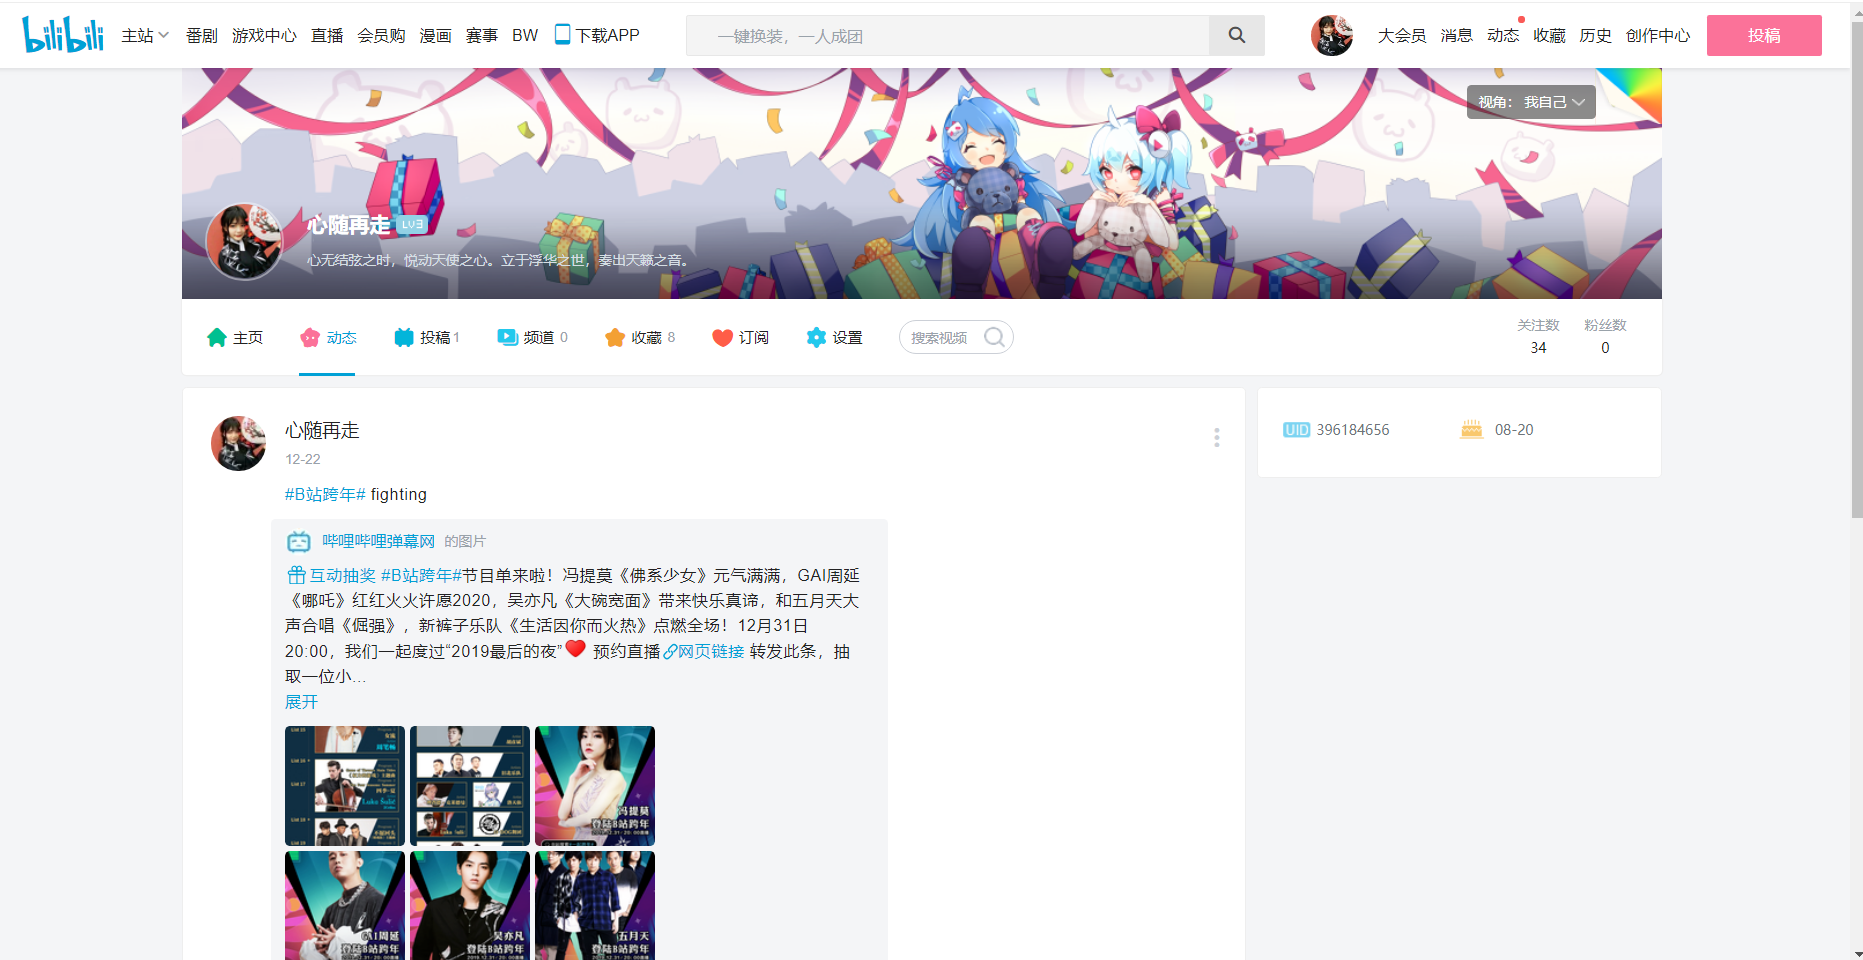
\includegraphics[scale=0.2]{1.5}
            \label{fig:1.5}
        \end{figure} 
    }
\newpage
    \item {
        \bf{CSDN}\\
        CSDN Blog: https://i.csdn.net/\#/uc/profile\\
        \begin{figure}[h]
            \centering
            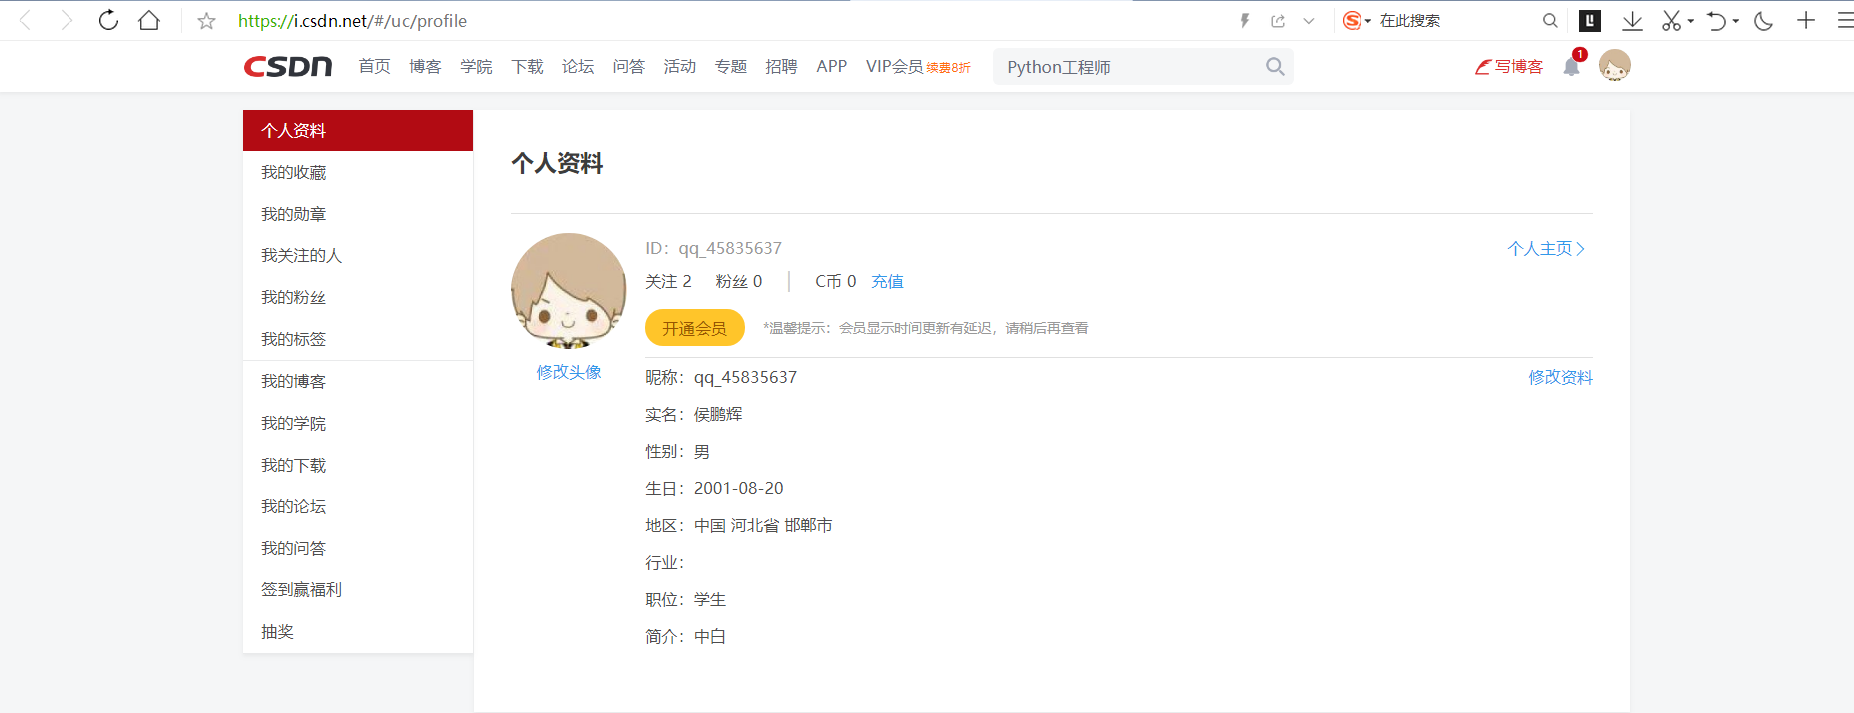
\includegraphics[scale=0.2]{1.6}
            \label{fig:1.6}
        \end{figure}
    }
    \item {
        \bf{博客园}\\
        https://www.cnblogs.com/Alneai/\\
        \begin{figure}[h]
            \centering
            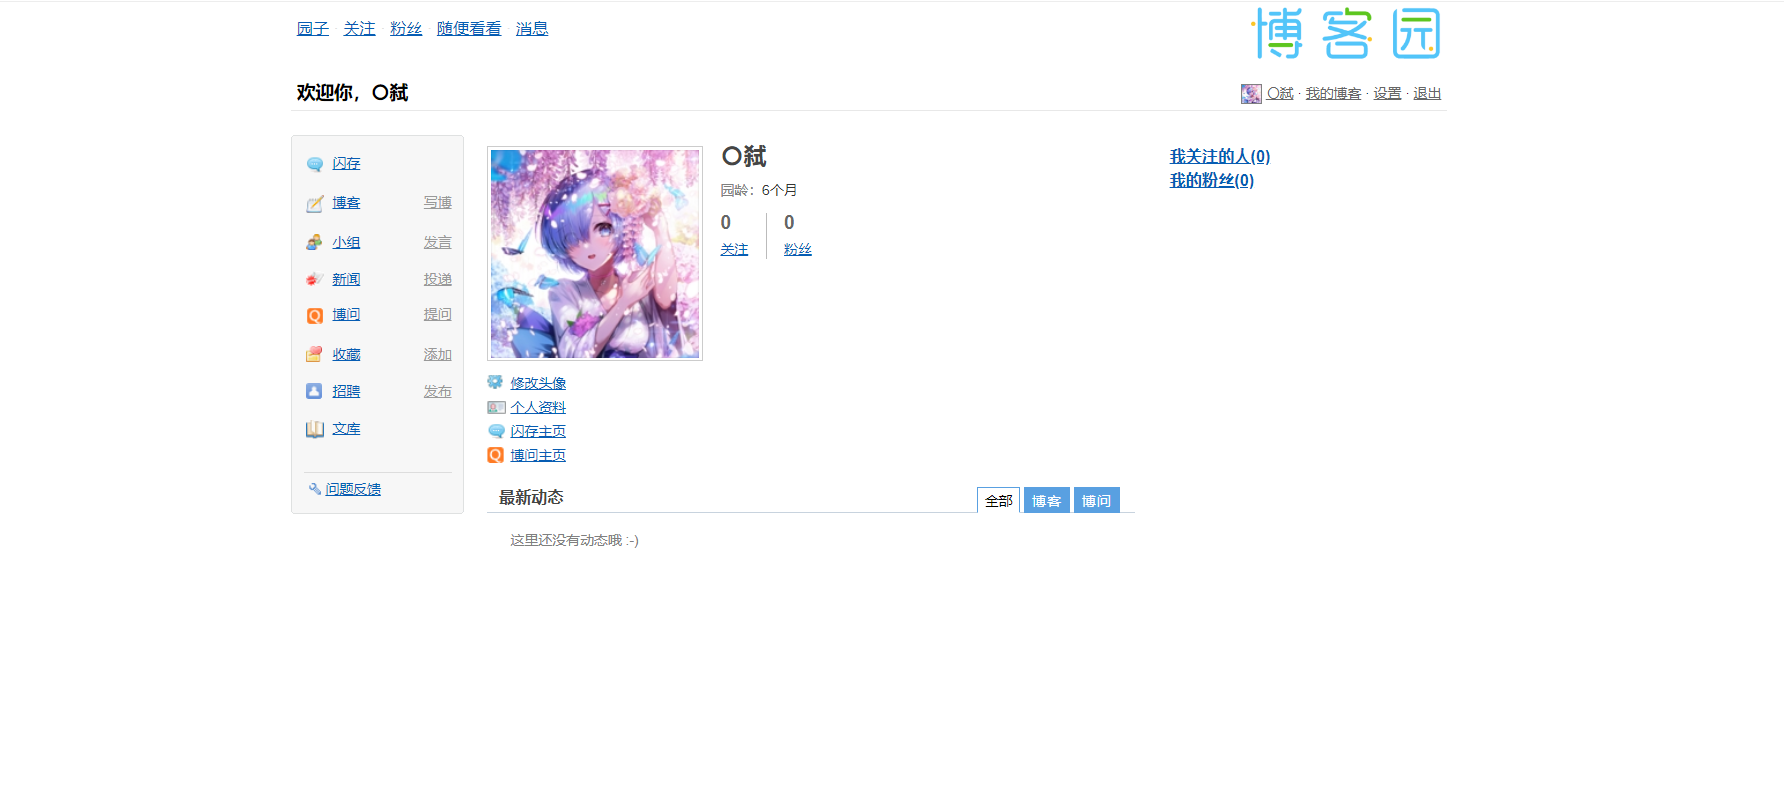
\includegraphics[scale=0.2]{1.7.1}
            \label{fig:1.7.1}
        \end{figure}
    }
    \item {
        \bf{小木虫}\\
        http://muchong.com/bbs/space.php?uid=20255786\\
        \begin{figure}[h]
            \centering
            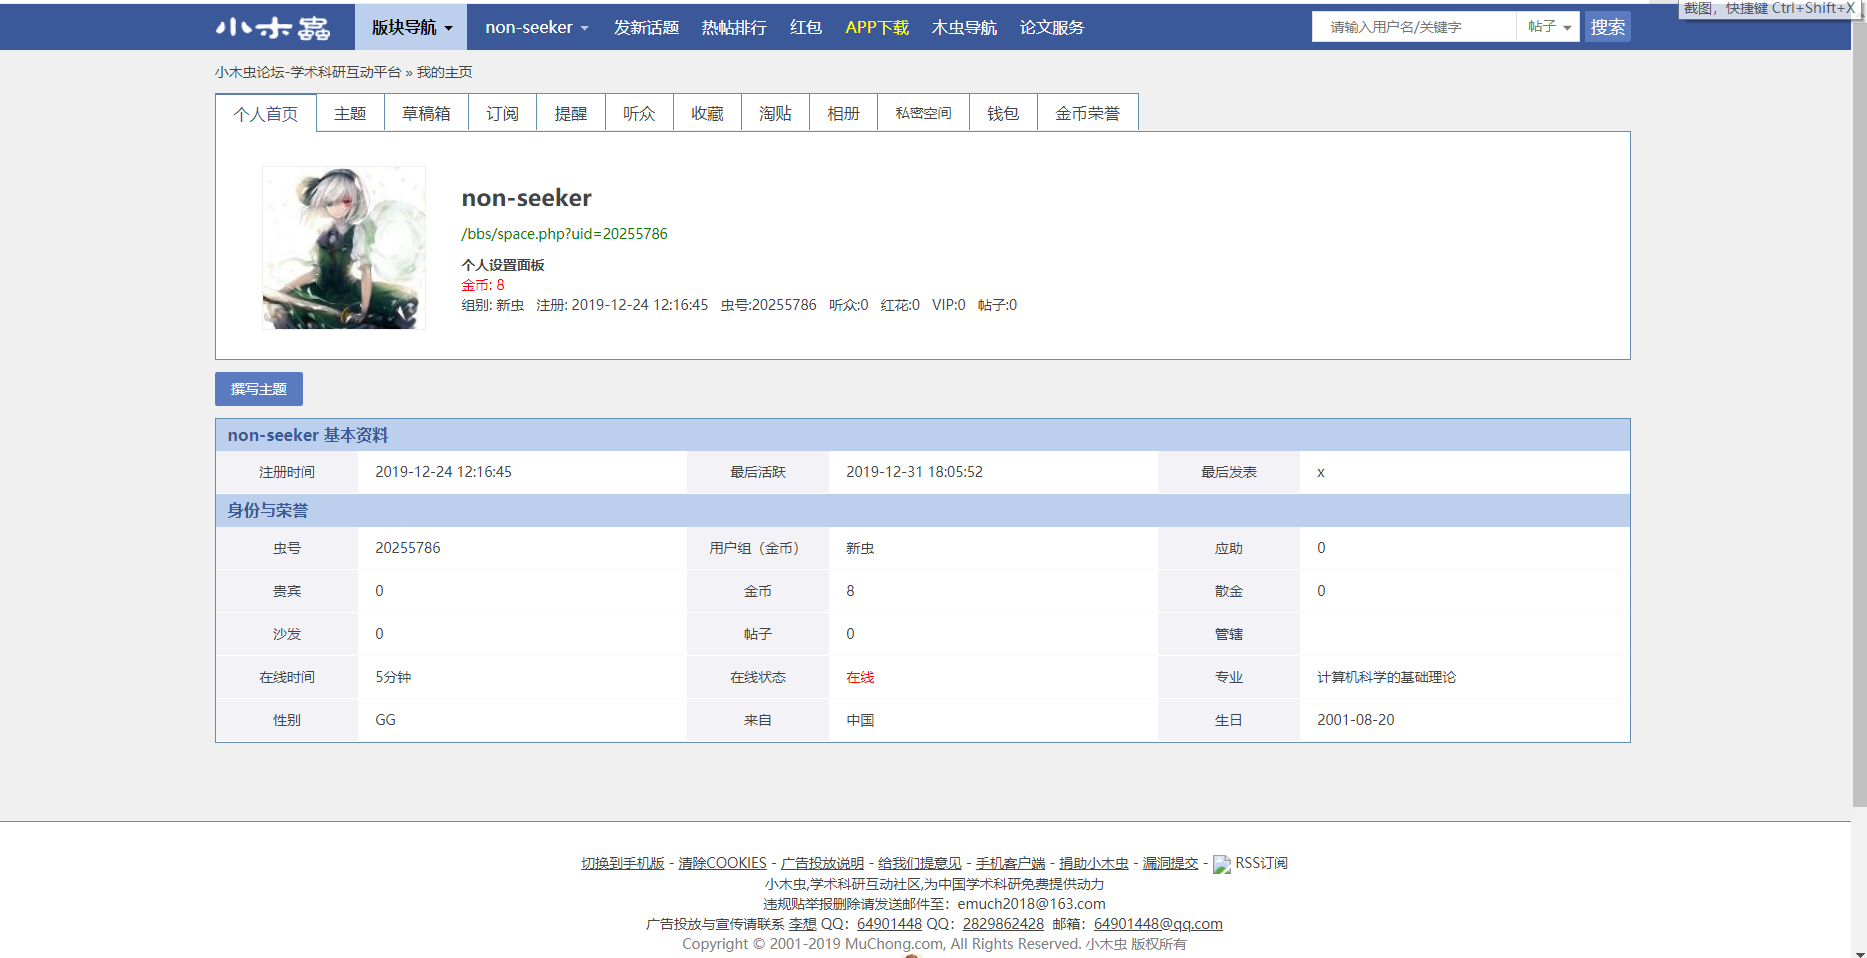
\includegraphics[scale=0.2]{1.8.1}
            \label{fig:1.8.1}
        \end{figure}
    }
\end{itemize}

\newpage

\bibliographystyle{plain}
\bibliography{references}
\begin{thebibliography}{99}  
    \bibitem{ref1} 来自彭博社Bloomberg的报道 \url{https://translate.google.com/translate?hl=zh-CN\&sl=en\&tl=zh-CN\&u=https\%3A\%2F\%2Fwww.cnet.com\%2Fnews\%2Fhuawei-exec-acknowledges-its-struggling-without-google-support\%2F\&anno=2 }
    \bibitem{ref2} 选自乌龟精神,追上龙飞船{任正非华为内部讲话实录} \url{https://passport.weibo.com/visitor/visitor?entry=miniblog\&a=enter\&url=https\%3A\%2F\%2Fweibo.com\%2F2162570295\%2FHjEYSca5n\%3Ftype\%3Dcomment\&domain=.weibo.com\&sudaref=https\%3A\%2F\%2Fwww.baidu.com\%2Flink\%3Furl\%3DzqpeRQE1FBWN2vbVv8lB4esQVTQDZa1aDzQyUry4GK5Ky5BHaQmcShPPVp0shAhR0I6NbmE_DM6GIPg23Nxdm_\%26wd\%3D\%26eqid\%3Dce4cdb000003fb13000000035e0adca3\&ua=php-sso_sdk_client-0.6.28\&_rand=1577770154.636>}
    \bibitem{ref3} 参考自 经济日报 \url{https://baijiahao.baidu.com/s?id=1641376146444125643&wfr=spider&for=pc}
    \bibitem{ref4} 百度知道 \url{https://baike.baidu.com/item/\%E9\%99\%88\%E6\%B5\%B7\%E6\%B3\%A2/16608320?fr=aladdin\#3>}
    \bibitem{ref5} 万物互联 | 华为全场景智慧化战略详解  \url{http://www.360doc.com/content/19/0422/20/2209670_830649033.shtml}
    \bibitem{ref6} 参考自 互联网浩浩 的 鸿蒙系统应该如何建立生态系统  \url{https://baijiahao.baidu.com/s?id=1636136445152788125\&wfr=spider\&for=pc>}
    \bibitem{ref7} 百度百科 \url{https://baike.baidu.com/item/\%E5\%8D\%8E\%E4\%B8\%BA\%E9\%B8\%BF\%E8\%92\%99\%E7\%B3\%BB\%E7\%BB\%9F/23500650?fr=aladdin}
\end{thebibliography}


\end{document}